%! TeX program = lualatex
\documentclass[]{beamer} 

\setbeamercolor{title}{fg=black}
\setbeamercolor{frametitle}{fg=black}
\setbeamercolor{caption}{fg=black}
\setbeamercolor{caption name}{fg=black}

\setbeamertemplate{navigation symbols}{}
\setbeamertemplate{itemize item}{\color{black}$\bullet$}

% packages
\usepackage{fontspec}
\setmainfont{EB Garamond}
\usefonttheme{serif}
\setmonofont[Scale=MatchLowercase]{Deja Vu Sans Mono}

\usepackage{microtype}      % Slightly tweak font spacing for aesthetics
\usepackage[english]{babel} % Language hyphenation and typographical rules

\usepackage{minted}
\usemintedstyle{algol_nu}
\usepackage{xcolor}

\usepackage{pgfplots}
\pgfplotsset{width=\textwidth,compat=1.9}

\usepackage{caption}
\newenvironment{code}{\captionsetup{type=listing, skip=0pt}}{}

\usepackage[yyyymmdd]{datetime}
\renewcommand{\dateseparator}{--}

\author{Andrew Hayes }
\title{CT437 Assignment 1}
\subtitle{Ethical Hacking \& Penetration Testing using Kali Linux \& Metasploit}
\institute{Student ID: 21321503}

\begin{document}

\frame{\titlepage}

\begin{frame}{Finding Exploits}
    The first thing I did to see what kind of vulnerabilities might exist in the Metasploitable2 virtual machine was to run a \mintinline{shell}{nmap} on the virtual machine's IP address to see what ports are in use and what services are on those ports:

\begin{figure}[H]
    \centering
    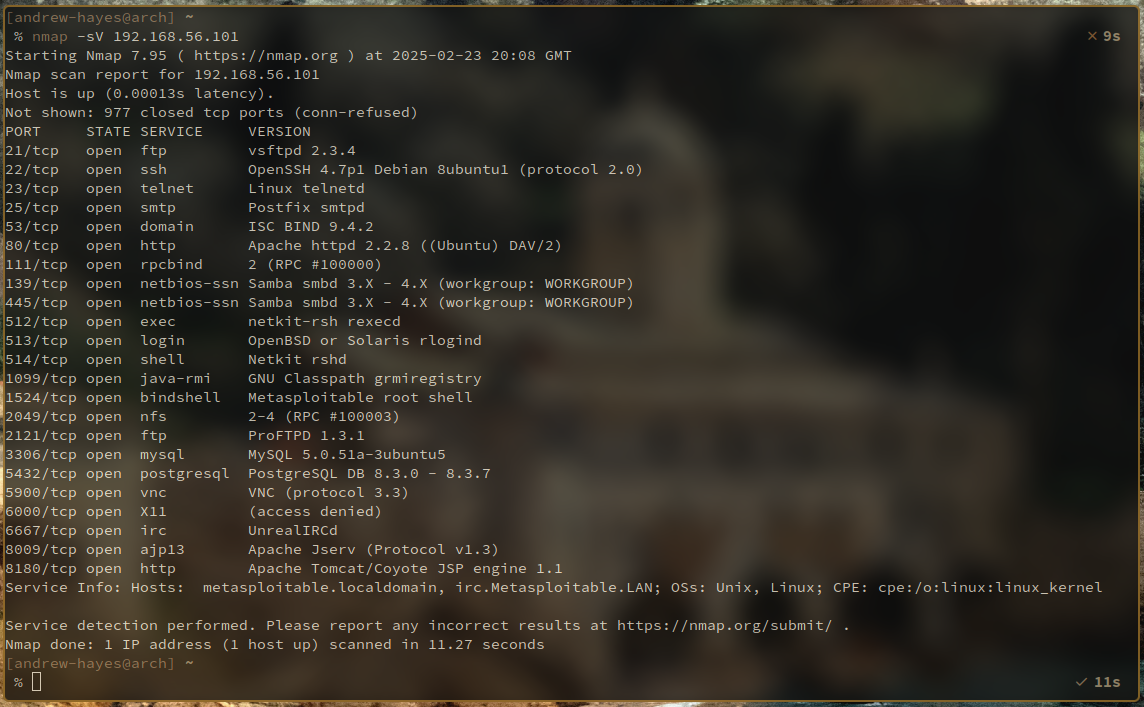
\includegraphics[width=0.8\textwidth]{./images/nmap.png}
    \caption{Output of \texttt{nmap}}
\end{figure}
\end{frame}

\begin{frame}{Exploit 1: FTP}
    Seeing that there was a FTP service running using \texttt{vsftpd 2.3.4}, I then searched for this service in the Metasploit console and saw that there was a backdoor exploit for this particular version of \texttt{vsftpd}:

\begin{figure}[H]
    \centering
    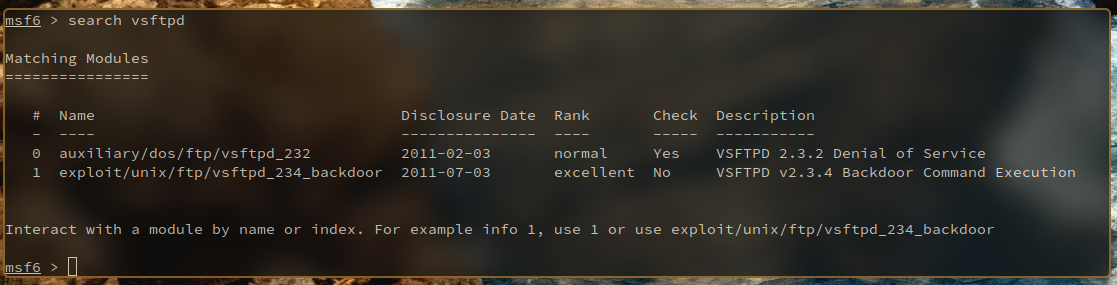
\includegraphics[width=\textwidth]{./images/searchftp.png}
    \caption{Output of \texttt{search vsftpd} in \texttt{msfconsole}}
\end{figure}
\end{frame}

\begin{frame}{Exploit 1: FTP}
    I then set the \texttt{RHOST} value and ran the exploit:

\begin{figure}[H]
    \centering
    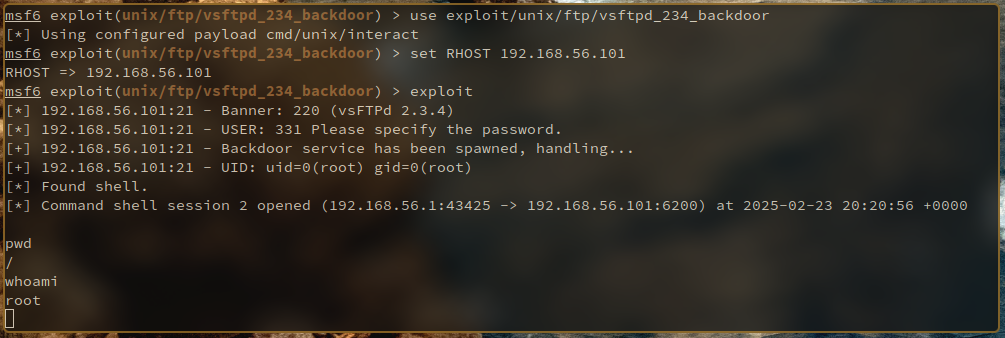
\includegraphics[width=\textwidth]{./images/ftpexploit.png}
    \caption{Results of running \texttt{use exploit/unix/ftp/vsftpd\_234\_backdoor}}
\end{figure}
\end{frame}

\begin{frame}{Exploit 1: FTP}
    \begin{itemize}
        \item   As can be seen from the output on the previous slide, this backdoor exploit gives us remote root access to the vulnerable Metasploitable2 machine -- a highly dangerous vulnerability.
        \item   This works because version \texttt{2.3.4} of the \texttt{vsftpd} program was shipped with a malicious backdoor inserted into the binary that is triggered when a user attempts to login with a username ending in \texttt{:)} and opens a command shell on TCP port \texttt{6200}.
        \item   The Metasploit exploit module attempts to login with a username ending in \texttt{:)}, triggering the backdoor, and then connects to port \texttt{6200}, thus giving the malicious user root access to the target system.
    \end{itemize}
\end{frame}

\begin{frame}{Exploit 2: Samba}
    Seeing from the \texttt{nmap} output that there is a Samba service running, I then searched for this service in the Metasploit console and saw that there were more than 70 possible exploits using Samba.
    One in particular caught my eye, that being the \texttt{exploit/multi/samba/usermap\_script} module, as it had rank ``Excellent'' and allows the attacker to gain shell access to the target system.
\end{frame}

\begin{frame}{Exploit 2: Samba}
    If you run \texttt{use exploit/multi/samba/usermap\_script} and then \texttt{show payloads} to see what payloads are available, 
    you will get a list of 44 payloads.

\begin{figure}[H]
    \centering
    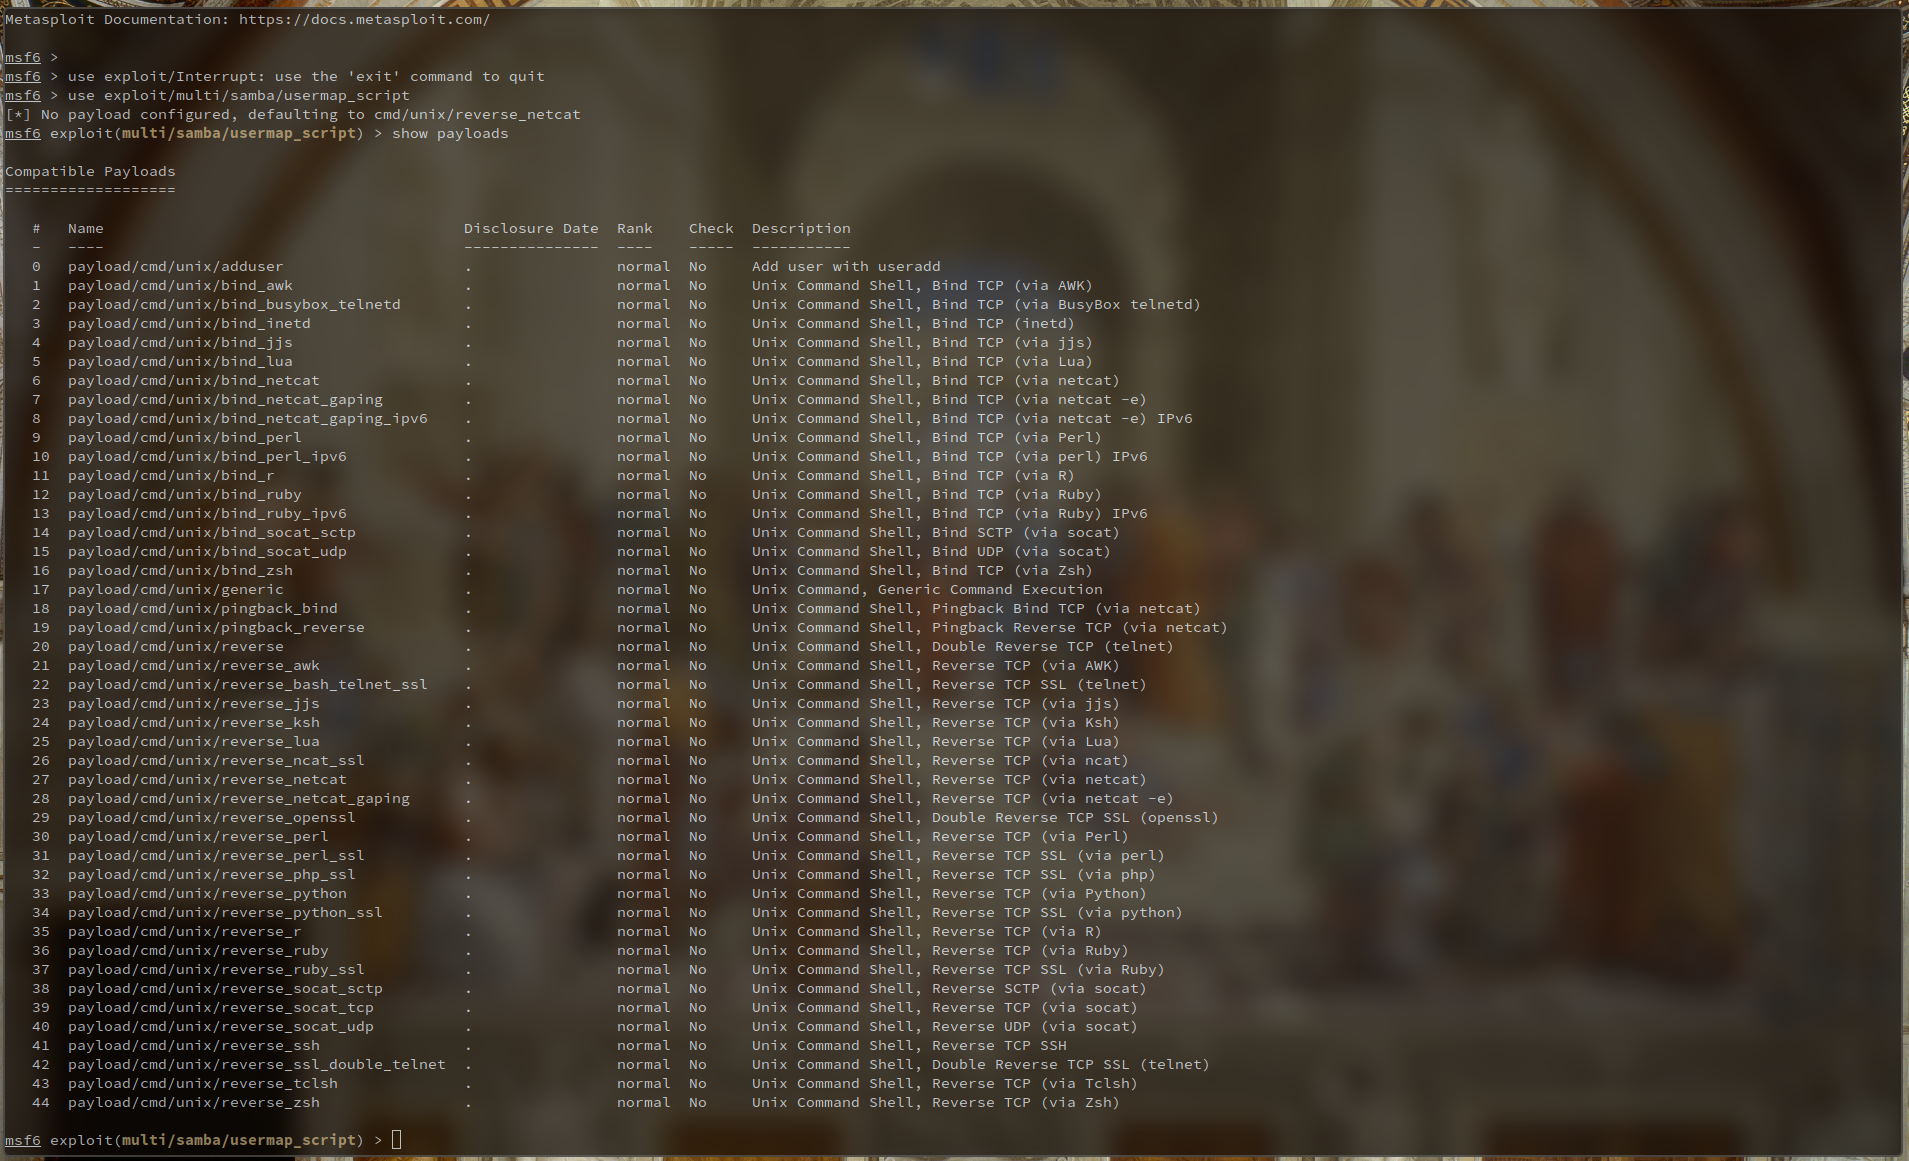
\includegraphics[width=\textwidth]{./images/sambapayloads.png}
    \caption{Available payloads}
\end{figure}

\end{frame}

\begin{frame}{Exploit 2: Samba}
I chose the payload \texttt{payload/cmd/unix/bind\_netcat}, which spawns a shell on the target machine and binds it to a port with \texttt{netcat}, allowing the attacker to connect.
I then set the \texttt{RHOST} and ran the exploit.

\begin{figure}[H]
    \centering
    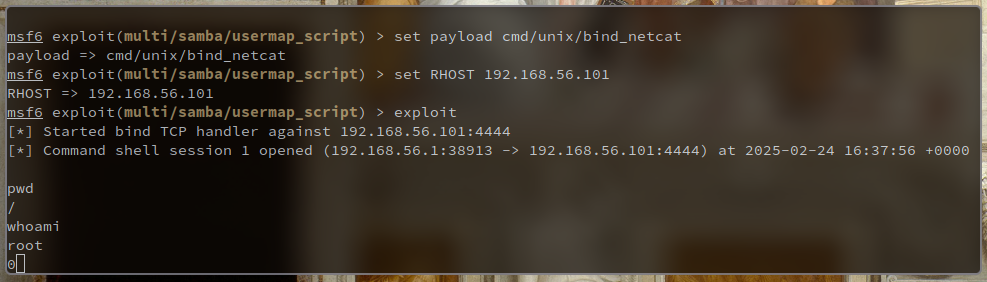
\includegraphics[width=\textwidth]{./images/sambaexploit.png}
    \caption{Running the exploit with \texttt{bind\_netcat} payload}
\end{figure}
\end{frame}

\begin{frame}{Exploit 2: Samba}
    \begin{itemize}
        \item   As can be seen from the output on the previous slide, this backdoor also gives us remote root access to the target machine.
        \item   This exploit works because Samba allows administrators to map incoming usernames to different local users using the \texttt{username map} feature, which processes the incoming usernames using a shell command.
        \item   In certain vulnerable versions of Samba, the user input is not sanitised properly and an attacker can insert special characters to inject arbitrary shell commands, such as spawning a \texttt{netcat} shell on a specific port.
    \end{itemize}
\end{frame}

\begin{frame}{Exploit 3: \texttt{distcc}}
    
\end{frame}

\end{document}
